%!TEX root = ../Master.tex

\section{Simulation} % (fold)
\label{sec:simulation}

For faster development of the algorithms we simulated the real robot instead of running the program on the actual robot. A particle was used as the simulated robot and measurement noise was added on the particles laser scans to simulate the real lidar. \\

The project works with large data sets, ie. 4000 particles, a map of 48*150 grid cells and 360 laser range measurments. These data sets are hard to understand without proper tools to visualizing the data in a intuitive way. To visualize the data the ROS tool RVIZ was used. RVIZ can subscribe to ROS topics and draw some standard ROS message types.\\

The data was displayed as \autoref{fig:rviz_close} shows. The simulated robot is shown as the green arrow head. The estimate is shown as the red arrow head, which at the time of the screenshot is right on top of the simulated robot. The particles are drawn as small green arrows that illustrates the position and orientation of the particle. The simulated lidar scan is shown as the red squares. Each red square illustrates what the laser scan hits.\\

The map is drawn in grayscale and the different shades of gray illustrates different costs of the map. The black parts of the map are walls, the dark gray are non accessable areas, the light gray are the floor, and the white are the preffered parts of the floor for path planning.\\

In \autoref{fig:rviz_follow} the 3D capability in RVIZ is shown. The camera will follow the robot around as it drives. In \autoref{fig:rviz_top} the RVIZ tool window with the entire map visible is shown.

\begin{figure}[H]
\centering
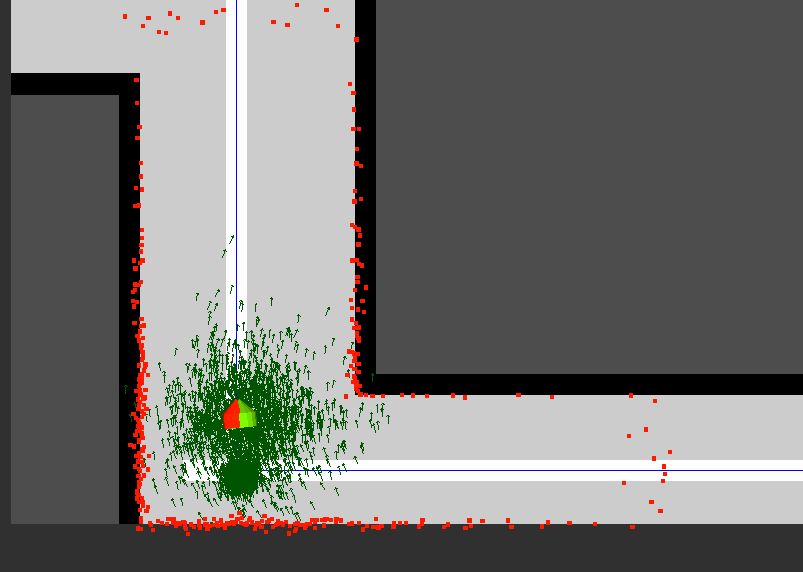
\includegraphics[scale=0.50]{images/rviz_close}
\caption{Top-down view. Shows how the data is displayed.}
\label{fig:rviz_close}
\end{figure}

\begin{figure}[H]
\centering
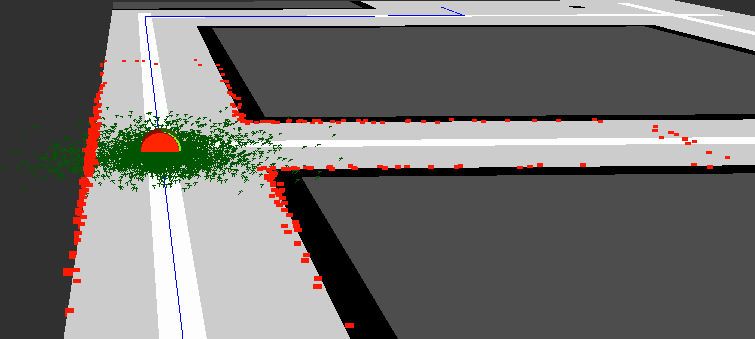
\includegraphics[scale=0.50]{images/rviz_follow}
\caption{3rd person view. 3D visualization where the camera follows the robot.}
\label{fig:rviz_follow}
\end{figure}

\begin{figure}[H]
\centering
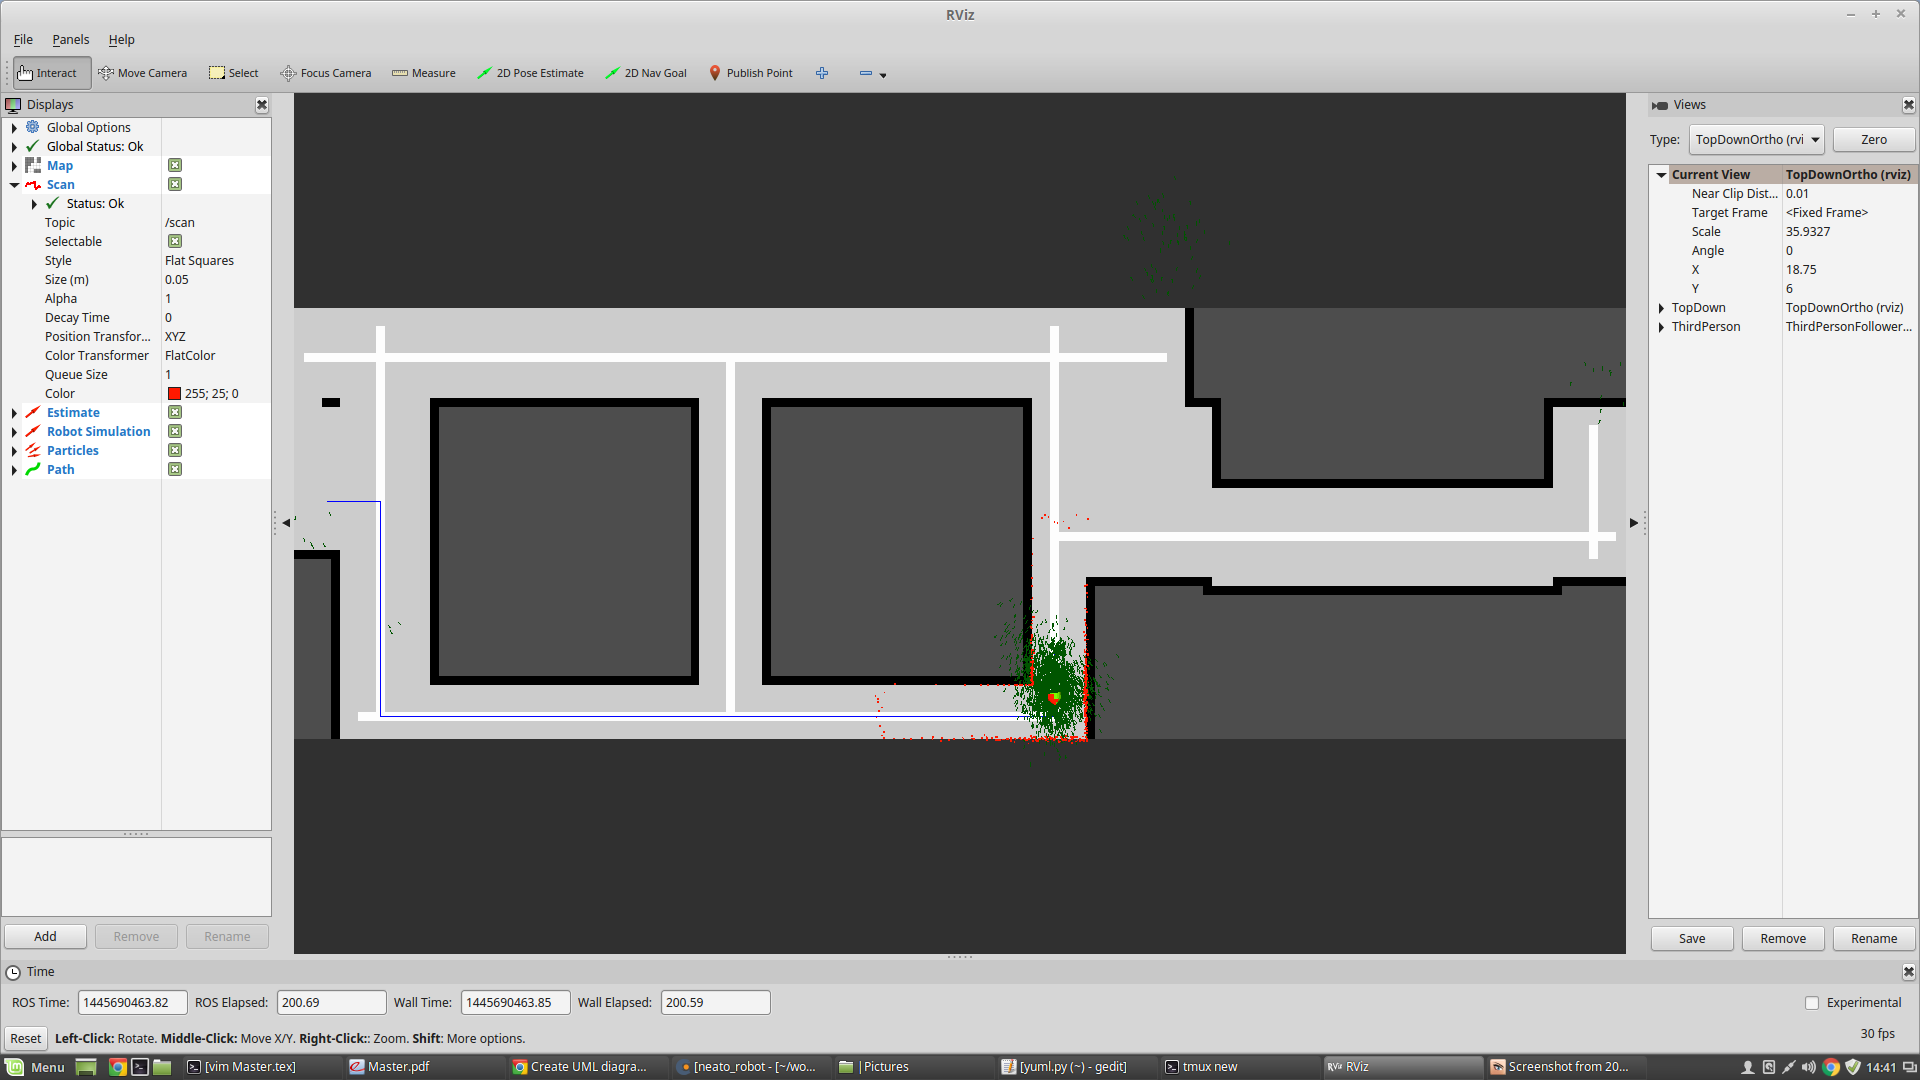
\includegraphics[scale=0.20]{images/rviz_top}
\caption{Top-down view. Overview of entire map.}
\label{fig:rviz_top}
\end{figure}
% section simulation (end)
